\documentclass[tikz,border=8pt]{standalone}
% Shared look for every TikZ diagram. Load with \input{../../tools/tikz-style.tex}
\usepackage[T1]{fontenc}
\usepackage{lmodern}
\renewcommand{\sfdefault}{lmr}  % diagrams use the same serif as the text
\usetikzlibrary{arrows.meta, positioning, shapes.geometric, calc, fit, backgrounds}
\definecolor{cblue}{HTML}{4C78A8}
\definecolor{corange}{HTML}{F58518}
\definecolor{cgreen}{HTML}{54A24B}
\definecolor{cred}{HTML}{E45756}
\definecolor{cpurple}{HTML}{B279A2}
\definecolor{cgrey}{HTML}{6B6B6B}
\tikzset{
  every picture/.style={font=\sffamily, line width=1.2pt},
  box/.style={draw=#1, fill=#1!12, rounded corners=4pt, align=center, inner sep=7pt, minimum height=1.1cm},
  box/.default=cgrey,
  arrow/.style={-{Stealth[length=3mm]}, draw=cgrey, line width=1.4pt},
  title/.style={font=\sffamily\bfseries\Large},
  note/.style={font=\sffamily\small, text=cgrey, align=center},
}
\AtBeginDocument{\hyphenpenalty=10000 \exhyphenpenalty=10000}

\begin{document}
% Section 6: the first show of the saved TVmaze reply (data/tvmaze_shows_page0.json). pd.DataFrame keeps the nested
% rating dictionary in one cell; pd.json_normalize opens it into its own column, rating.average.
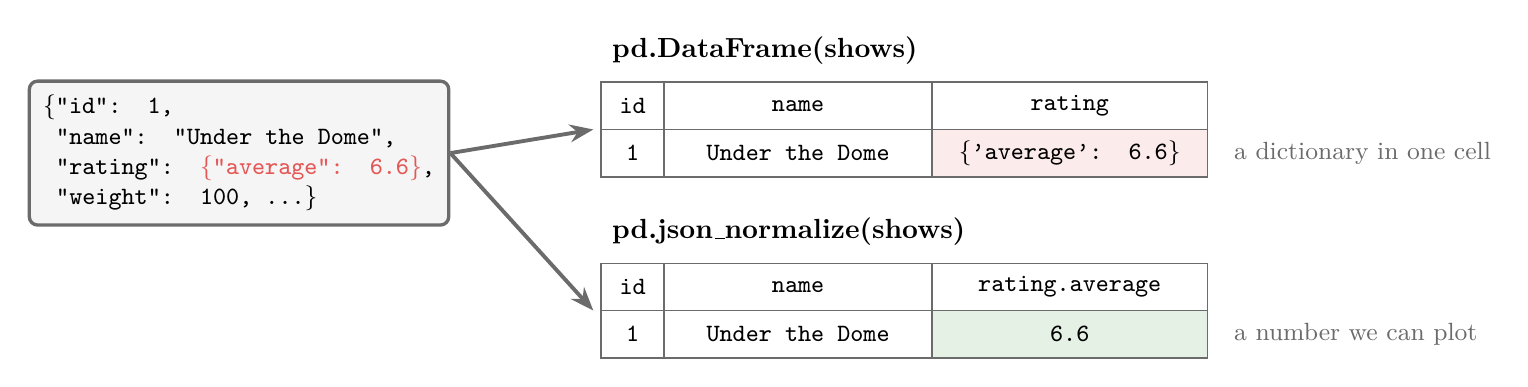
\begin{tikzpicture}[c/.style={draw=cgrey, minimum height=0.6cm, font=\ttfamily\small, line width=0.6pt, inner sep=3pt},
  j/.style={draw=cgrey, fill=black!4, rounded corners=3pt, font=\ttfamily\small, align=left, inner sep=5pt}]
  \node[j] (js) at (0, 0) {\{"id": 1,\\\ "name": "Under the Dome",\\\ "rating": \textcolor{cred}{\{"average": 6.6\}},\\\ "weight": 100, \dots\}};
  \node[font=\sffamily\bfseries, anchor=west] at (4.6, 1.3) {pd.DataFrame(shows)};
  \node[c, minimum width=0.8cm] at (5.0, 0.6) {id}; \node[c, minimum width=3.4cm] at (7.1, 0.6) {name}; \node[c, minimum width=3.5cm] at (10.55, 0.6) {rating};
  \node[c, minimum width=0.8cm] at (5.0, 0.0) {1}; \node[c, minimum width=3.4cm] at (7.1, 0.0) {Under the Dome}; \node[c, minimum width=3.5cm, fill=cred!12] at (10.55, 0.0) {\{'average': 6.6\}};
  \node[font=\sffamily\bfseries, anchor=west] at (4.6, -1.0) {pd.json\_normalize(shows)};
  \node[c, minimum width=0.8cm] at (5.0, -1.7) {id}; \node[c, minimum width=3.4cm] at (7.1, -1.7) {name}; \node[c, minimum width=3.5cm] at (10.55, -1.7) {rating.average};
  \node[c, minimum width=0.8cm] at (5.0, -2.3) {1}; \node[c, minimum width=3.4cm] at (7.1, -2.3) {Under the Dome}; \node[c, minimum width=3.5cm, fill=cgreen!15] at (10.55, -2.3) {6.6};
  \draw[arrow] (js.east) -- (4.5, 0.3); \draw[arrow] (js.east) -- (4.5, -2.0);
  \node[note, anchor=west] at (12.5, 0.0) {a dictionary in one cell};
  \node[note, anchor=west] at (12.5, -2.3) {a number we can plot};
\end{tikzpicture}
\end{document}
